\begin{solution}
\begin{enumerate}
\item {[5 points]} Integration by parts yields that
\begin{eqnarray*}
&&a\ip{u_m,u_m}
\\
&=&\int_0^1{d \over dx}\left(\sqrt{2}\sin\left(m\pi x\right)\right){d \over dx}\left(\sqrt{2}\sin\left(m\pi x\right)\right)\,dx
\\
&=&\left[{d \over dx}\left(\sqrt{2}\sin\left(m\pi x\right)\right)\sqrt{2}\sin\left(m\pi x\right)\right]_0^1-\int_0^1{d^2 \over dx^2}\left(\sqrt{2}\sin\left(m\pi x\right)\right)\sqrt{2}\sin\left(m\pi x\right)\,dx
\\
&=&\left[2m\pi\cos\left(m\pi x\right)\sin\left(m\pi x\right)\right]_0^1+\int_0^1\sqrt{2}m^2\pi^2\sin\left(m\pi x\right)\sqrt{2}\sin\left(m\pi x\right)\,dx
\\
&=&2m\pi\cos\left(m\pi\right)\sin\left(m\pi\right)-2m\pi\cos\left(0\right)\sin\left(0\right)+m^2\pi^2\ip{u_m,u_m}
\\
&=&m^2\pi^2\ip{u_m,u_m}
\end{eqnarray*}
since $\sin\left(0\right)=0$ and $\sin\left(m\pi\right)=0$ when $m$ is a positive integer. Therefore, the fact that $\ip{u_m,u_m}=1$ allows us to conclude that
\[
a\ip{u_m,u_m}=m^2\pi^2.
\]
\\
\item {[10 points]} The code for this part and part (c) is:

\lstinputlisting{HW34.m}

The requested plot is below.

\begin{center}
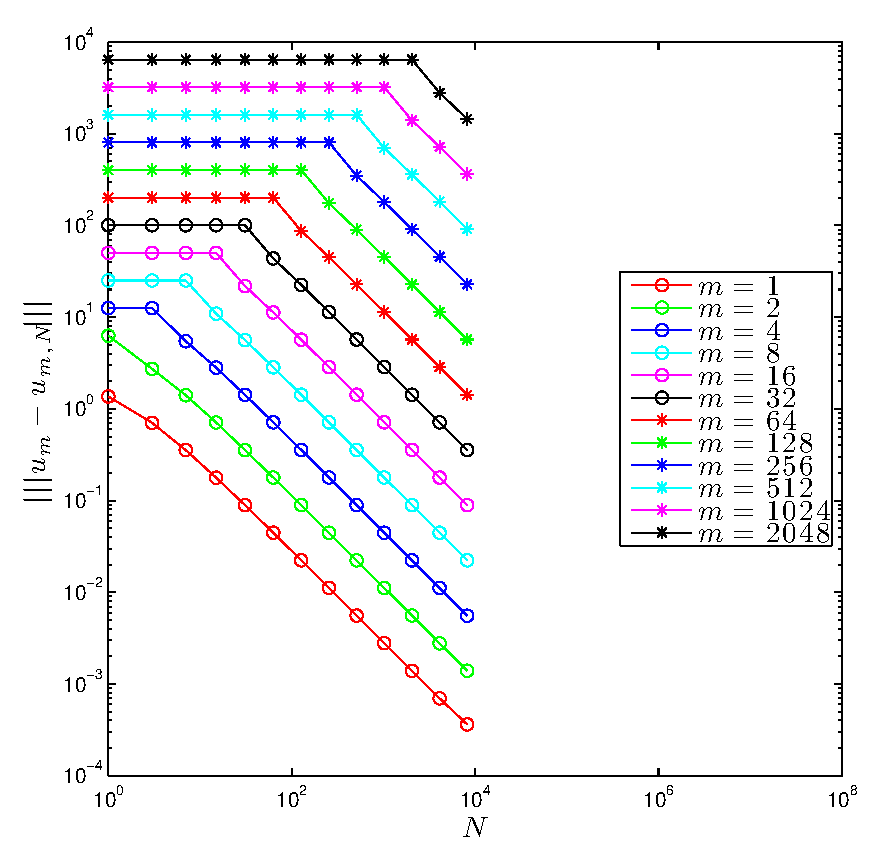
\includegraphics[scale=0.75]{hw34b.eps}
\end{center}

\item {[5 points]} The requested plot is below.

\begin{center}
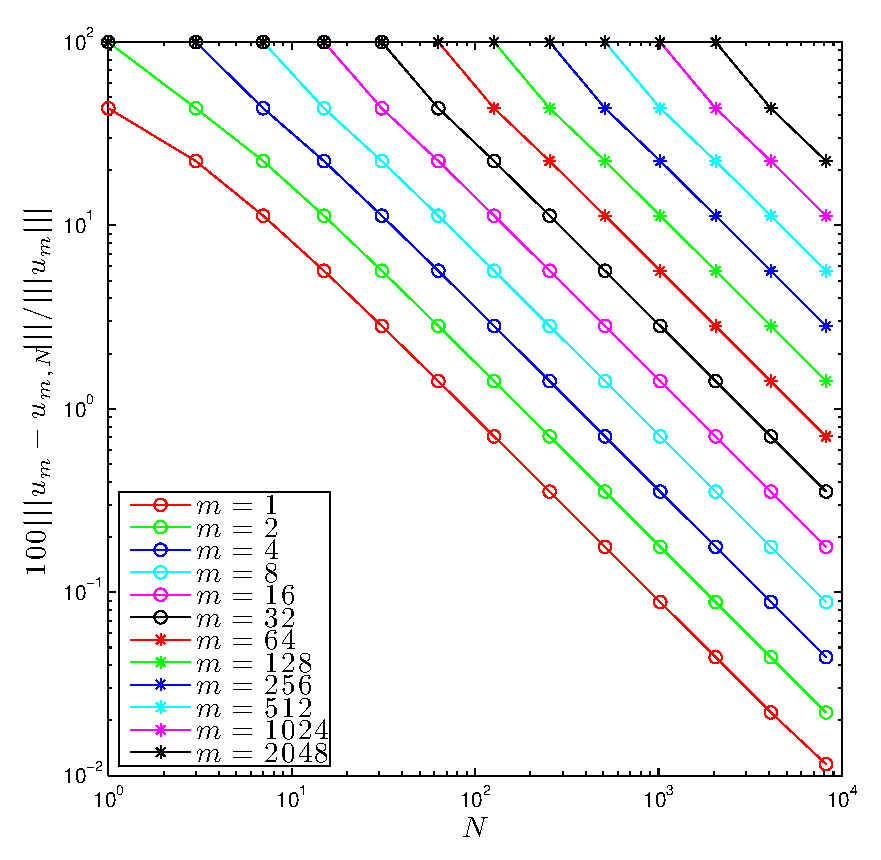
\includegraphics[scale=0.75]{hw34c.eps}
\end{center}

\item {[5 points]} For $j=0,\ldots,N$, when $x\in(x_j,x_{j+1})$, $\phi_k''(x)=0$ for $k=1,\ldots,N$. Hence, if $\tilde{u}_N\in V_N$ then for $j=0,\ldots,N$, when $x\in(x_j,x_{j+1})$, $\tilde{u}_N''(x)=0$. Therefore,
\[
\sum_{j=0}^N\int_{x_j}^{x_{j+1}}(f(x)+\tilde{u}_N''(x))^2\,dx=\sum_{j=0}^N\int_{x_j}^{x_{j+1}}(f(x))^2\,dx=\int_0^1(f(x))^2\,dx
\]
for all $\tilde{u}_N\in V_N$. So, if $\tilde{u}_N\in V_N$, then the value of
\[
\sum_{j=0}^N\int_{x_j}^{x_{j+1}}(f(x)+\tilde{u}_N''(x))^2\,dx
\]
does not change as $N$ increases as for all positive integers $N$
\[
\sum_{j=0}^N\int_{x_j}^{x_{j+1}}(f(x)+\tilde{u}_N''(x))^2\,dx=\int_0^1(f(x))^2\,dx.
\]
\end{enumerate}
\end{solution}